\documentclass[a4paper, bibgerm]{article}
\usepackage[utf8]{inputenc}
\usepackage[T1]{fontenc}
\usepackage{lmodern}
\usepackage{ngerman}
\usepackage{bibgerm}
\usepackage{color}
\usepackage{amsfonts}
\usepackage{graphicx}
\usepackage{subfig}
% \usepackage{pstricks}
% \usepackage{pst-node}
\usepackage{hyperref}

\newcommand{\defaultscale}{0.3}

\newcommand\lsection{}
\newcommand\lsubsection{}
\newcommand\lsubsubsection{}
\newcommand\lparagraph{}
\newcommand\sref{}
\newcommand\abb{}
\newcommand\fig{}
\newcommand\figs{}
\newcommand\subfig{}
\newcommand\vertfig{}
\newcommand\clipvertfig{}

\newcommand{\project}[1]{%
  \renewcommand\lsection[2][\LSectionDefault]{%
    \def\LSectionDefault{##2}%
    \section{##2}
    \label{#1:sec:##1}%
  }
  \renewcommand\lsubsection[2][\LSubSectionDefault]{%
    \def\LSubSectionDefault{##2}%
    \subsection{##2}
    \label{#1:sec:##1}%
  }
  \renewcommand\lsubsubsection[2][\LSubSubSectionDefault]{%
    \def\LSubSubSectionDefault{##2}%
    \subsubsection{##2}
    \label{#1:sec:##1}%
  }
  \renewcommand\lparagraph[2][\LParagraphDefault]{%
    \def\LParagraphDefault{##2}%
    \paragraph{##2}
    \label{#1:sec:##1}%
  }  
  \renewcommand\sref[1]{%
    Abschnitt~\ref{#1:sec:##1}
  }%
  \renewcommand{\abb}[1]{Abb.\ref{#1:fig:##1}}
  \renewcommand{\fig}[3][\defaultscale]{%
    \begin{figure}[htp]
      \centering
      \includegraphics[scale=##1]{images/##2}
      \caption{##3}
      \label{#1:fig:##2}
  \end{figure}}

  \renewcommand{\figs}[2]{%
    \begin{figure}[htp]
      \centering
      ##2
      \caption{##1}
    \end{figure}
  }

  \renewcommand{\subfig}[3][\defaultscale]{%
    \subfloat[##3]{
      \includegraphics[scale=##1]{images/##2}
      \label{#1:fig:##2}
    }
  }

  \renewcommand{\vertfig}[3][\defaultscale]{%
    \begin{sidewaysfigure}[htp]
      \centering
      \includegraphics[scale=##1]{images/##2}
      \caption{##3}
      \label{#1:fig:##2}
    \end{sidewaysfigure}%
  }

  \renewcommand{\clipvertfig}[5]{%
    \begin{sidewaysfigure}[htp]
      \centering
      \includegraphics*[scale=##1, viewport=##2]{images/##3}
      \caption{##5}
      \label{#1:fig:##4}
    \end{sidewaysfigure}%
  }
}

\project{magicl}

\newcommand\code[1]{\texttt{#1}}
\newcommand\ato{\rightarrow}

\newtheorem{defi}{Definition}

\begin{document}

\title{MagicL: Ein Arrow-basiertes Compilerbau-Framework}
\author{Benjamin Teuber}
\date{\today}

% \maketitle

\begin{abstract}
  MagicL ist der Prototyp eines universellen Frameworks für den Entwurf
  von Programmier- und Auszeichnungssprachen. Es soll dem
  Meta-Programmierer praktische Werkzeuge für das Parsing und Übersetzen
  neuer sowie für Generation von Code bestehender Sprachen an die Hand
  geben, wobei insbesondere (jedoch nicht ausschließlich) aus
  S-Expressions aufgebaute Sprachen unterstützt werden. Die Parser- und
  Compilererstellung erfolgt nach einem kategorientheoretisch
  motivierten Baukastenansatz, so dass beispielsweise Parser durch die
  Kombination von Arrows erzeugt werden.
\end{abstract}

% \tableofcontents

\section{Einleitung}
\label{sec:intro}

Modellgetriebene Softwareentwicklung ist in aller Munde: Während UML
bald sein 20-Jähriges Jubiläum \footnote{Zumindest was die ersten
  Entwürfe angeht - der Standardisierungsprozess war erst 1997
  abgeschlossen.} feiert, verspricht Microsoft mit \textit{Oslo}
\cite{TODO} einen ``Mainstream-Ansatz für Modellierung''. IBM vermarktet
seit Jahren \textit{Rational Application Developer}, das wie auch das
freie \textit{Eclipse Modelling Framework} oder auch \textit{Enterprise
  Architect} Eclipse um modellbasierte Codegenerierung bereichern.
Code-Generation fällt auch im World Wide Web eine immer größer werdende
Rolle zu: Ob \textit{Ruby on Rails} oder \textit{Google Web Toolkit},
praktisch alle Web Frameworks generieren zumindest ihre HTML-Dateien oder
SQL-Strings für den Datenbankzugriff.

Der ganze Bereich um Code-Generation ist also ein aktuelles Thema.

\subsection{Codegenerierung}
\label{sec:intro:codegen}

Allgemein ist jedermann klar, was Codegenerierung bedeutet:
Das automatisiertes Erzeugen von Quelltext. Dennoch gibt es diverse
Unterschiede zwischen Codegenerierungswerkzeugen.

So differenziert man zwischen aktiver und passiver
Codegenerierung. Aktiv bedeutet, dass die Generierung wiederholt
ausgeführt werden kann, wenn sich etwas am Modell oder Generator ändert,
da die komplette Datei generiert wird. Passiv generierter Code dagegen
wird anschließend vom Programmierer modifiziert bzw. erst mit sinnvollen
Inhalten bestückt, so dass dieser nur normalerweise nur einmalig
generiert werden kann, wenn die Anpassungen nicht überschrieben werden
sollen. Zwischen aktiver und passiver Generierung liegen Dateien, in
denen nur markierte Abschnitte generiert werden - so dass der Rest
unverändert bleiben kann. Optimal wäre natürlich ein allgemeiner
Merge-Mechanismus, der die Arbeit des Programmierers reibungslos in die
neue Version übernimmt - dies ist aber leider schwierig zu
implementieren.

Zudem lässt sich nach Ein- und Ausgabe des Generators unterscheiden.

Vorteile:
\begin{itemize}
\item Abstraktion - Modellarchitekten beötigen keine
  Programmiersprachkenntnisse, Backend austauschbar
``Ist die Sprache an die Problemdomäne angepasst, muss man das Problem
nicht in die Sprache zwängen''
\item Produktivität - DRY-Prinzip spart u.U. viel Zeit
\item Qualität - ist der Generator fehlerfrei, gibt es keine Probleme
  bei neuen Modellen
\item Konsistenz - einheitliche Strukturen/Namen, minimiert Einarbeitungszeit
\end{itemize}

Nachteile:
\begin{itemize}
\item Dokumentation / Einarbeitung
\item Fehlersuche
\item Komplexität
\item Entwicklungsaufwand
\end{itemize}

\subsection{Lisp}
\label{sec:into:lisp}

-Code-Generation und Metaprogrammierung seit fast 50 Jahren
-was können wir lernen?
--Einheitliche Syntax macht vieles leichter
--compilererweitungen durch makros

\subsubsection{Vergleich mit XML}
\label{sec:intro:lisp:xml}

-gleiche Zielsetzung - Baumstruktur
-syntax: ``</tag>'' vs. ``)''
--nur vorteilhaft f texteditor ohne parent-matching!
-XML komplexer, da Attribute
--kann auch durch unterknoten ausgedrückt werden - wird es nur aufgrund
von hässlicher syntax nicht
--nicht mehr rekursiv, komplexe attribute gehen nicht (wirklich)

diskussion: makros good or bad

\subsection{Zielsetzung}
\label{sec:intro:goal}

\section{Erster Prototyp in Ruby}
\label{sec:sexy}

\section{Arrow-basierte Implementation in Haskell}
\label{sec:magicl}

\subsection{Kategorientheoretische Grundlagen}
\label{sec:magicl:cats}

Die Kategorientheorie ist ein sehr abstrakter Zweig der Mathematik -
aber auch ein universeller, denn fast alle wichtigen mathematischen
Strukturen sind Kategorien. Kategorientheorie findet dank seiner
Allgemeinheit und Anwendbarkeit für Berechnungen auch in der Informatik
eine immer größer werdende Rolle. Die Implementation von MagicL benutzt
einige kategorientheorietische Begriffe , z.B. werden Parser als
zusammengesetzte Funktoren konstruiert. Dieser Abschnitt führt in die
Kategorientheorie ein und stellt alle später verwendeten Konzepte
vor. Die Definitionen sind weitgehend aus \cite{Grundlagen} übernommen.

\fig[0.3]{cat_funs}{Ein simples Funktionensystem}

Der Grundansatz der Kategorientheorie ist die Verallgemeinerung der
Art und Weise, wie mit Funktionstypen gerechnet wird - insbesondere
hinsichtlich der Komposition von Funktionen. \abb{cat_funs} zeigt ein
kleines Funktionensystem zwischen den Mengen $\mathbb{R} \times
\mathbb{R}$, $\mathbb{R}$ und $\mathbb{Z}$. Es kommen folgende
Funktionen vor:
\begin{itemize}
\item $+ : \mathbb{R} \times \mathbb{R} \ato \mathbb{R}$ addiert zwei
  reelle Zahlen.
\item $\mathrm{abs} : \mathbb{R} \ato \mathbb{Z}$ ist die Betragsfunktion.
\item $+1 : \mathbb{Z} \ato \mathbb{Z}$ addiert $1$ zu einer ganzen Zahl.
\item $\mathrm{abs} \circ + : \mathbb{R} \times \mathbb{R} \ato \mathbb{Z}$
  addiert zwei reelle Zahlen und bildet anschließend den Betrag.
\end{itemize}

Die Komposition $\mathrm{abs} \circ +$ lässt sich bilden, weil der
Definitionsbereich von $\mathrm{abs}$ mit dem Zielbereich von $+$
übereinstimmt (nämlich $\mathbb{R}$). Es lassen sich also zwei im
Diagramm aufeinander folgende Pfeile zu einem direkten
zusammenfassen. Die Kategorientheorie "`vergisst"' nun den Bezug zu
Mengen und Funktionen und arbeitet statt dessen abstrakt mit Objekten
und Morphismen. 

\begin{defi}[Kategorie]
Eine Kategorie $\mathbf{C} = (\mathrm{Ob}^\mathbf{C}, \mathrm{Mor}^\mathbf{C},
\circ^\mathbf{C}, \mathrm{id}^\mathbf{C})$ ist gegeben durch 
\begin{itemize}
\item eine Klasse $\mathrm{Ob}^\mathbf{C}$ von Objekten\footnote{Da Objekte selbst Mengen
    sein können, wäre eine Definition von $\mathrm{Ob}^\mathbf{C}$ als Menge problematisch.}.
\item eine Menge Morphismen $\mathrm{Mor}^\mathbf{C}_{A,B}\forall A,B \in
  \mathrm{Ob}^\mathbf{C}$, wobei $A$ und $B$ Domäne und Codomäne genannt werden,
\item einen Kompositionsoperator $\circ^\mathbf{C}_{A,B,C}\forall
  A,B,C \in \mathrm{Ob}^\mathbf{C}$ mit \\
  $\circ^\mathbf{C}_{A,B,C} : \mathrm{Mor}^\mathbf{C}_{B,C} \times
  \mathrm{Mor}^\mathbf{C}_{A,B} \rightarrow \mathrm{Mor}^\mathbf{C}_{A,C}$,
\item eine Identität $\mathrm{id}^\mathbf{C}_A \in \mathrm{Mor}^\mathbf{C}_{A,A}\forall A \in \mathrm{Ob}^\mathbf{C}$,
\end{itemize}
wobei folgende Axiome erfüllt sein müssen:
\begin{itemize}
\item Neutralität der Identität: $$f \circ_{A,A,B} \mathrm{id}_A = \mathrm{id}_B \circ_{A,B,B} f = f$$
\item Assoziativität:
  $$f \circ_{A,C,D} (g \circ_{A,B,C} h) = (f \circ_{B,C,D} g) \circ_{A,B,D}h$$
\end{itemize}
\end{defi}


\begin{figs}{Kommutative Diagramme für die Kategorie-Axiome}
  \subfig{cat_id}{Identität}
  \subfig{cat_comp}{Assoziativität}
\end{figs}

% \begin{figure}
%   \centering
%   \subfloat[Identität]{
%     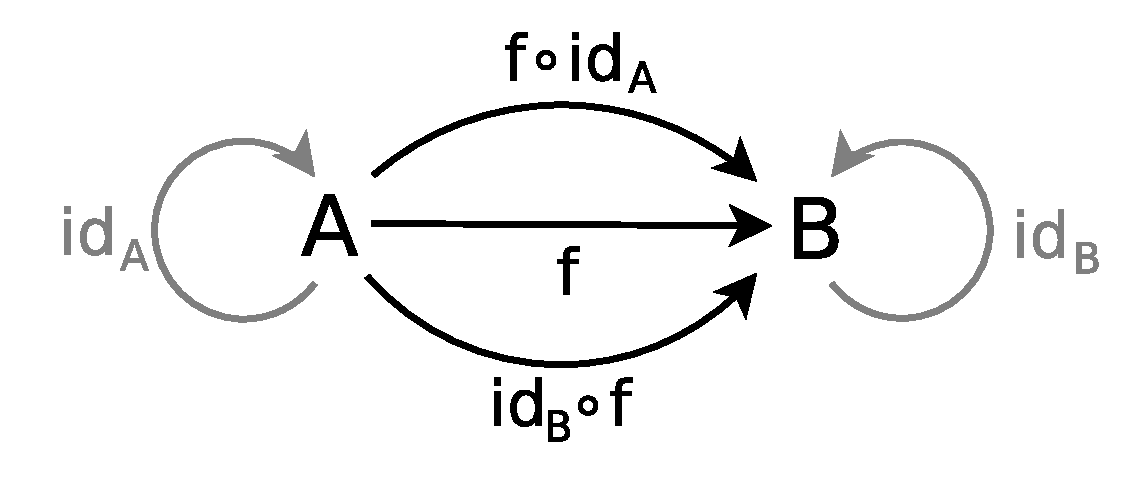
\includegraphics[scale=0.3]{images/cat_id}
%   }
%   \subfloat[Assoziativität]{
%     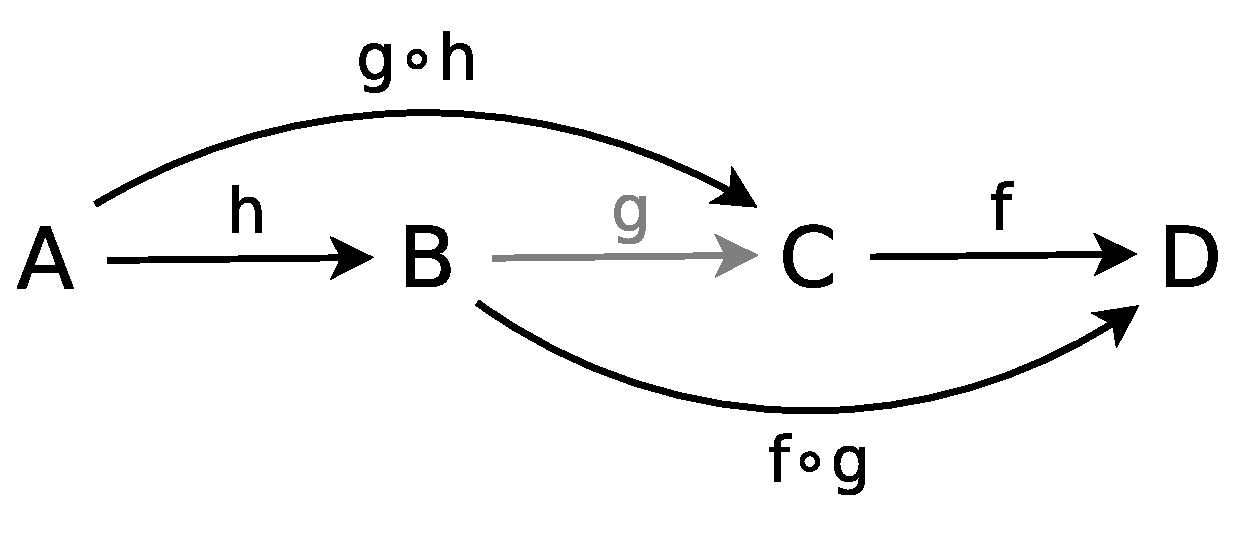
\includegraphics[scale=0.3]{images/cat_comp} 
%   }
%   \caption{Kommutative Diagramme für die Kategorie-Axiome}
%   \label{magicl:fig:cat_axioms}
% \end{figure}

Indizes und Kategorien werden der Einfachheit halber weggelassen, wenn
sie aus dem Kontext hervorgehen. Die Axiome lassen sich auch durch
kommutative Diagramme ausdrücken. Ein Diagramm kommutiert, wenn jeder
Pfad\footnote{Eine sinnvolle Definition des Begriffs "`Pfad"' und somit
  auch kommutative Diagramme setzen bereits Assoziativität von $\circ$
  voraus, weswegen die Diagramme hier ausschließlich der
  Veranschaulichung dienen und nicht bereits selbst - wie häufig in der
  Kategorientheorie - die Definition \textit{sind}.}  von $A$ nach $B$
durch Komposition zum selben Morphismus aus $\mathrm{Mor}_{A,B}$
verknüpft wird. Die Axiome bedeuten also, dass die Diagramme aus
\abb{cat_axioms} kommutieren. Die grauen Morphismen sind nur der
Vollständigkeit halber eingezeichnet.

\fig[0.3]{cat_simple}{Eine einfache Kategorie}

Wie das Einführungsbeispiel erwarten lässt, bilden die Mengen und
Funktionen eine Kategorie, genannt $\mathbf{Set}$. \abb{cat_simple} zeigt eine
andere simple Beispielkategorie, die aus den Objekten $A, B$ und den
Morphismen $f, g, \mathrm{id}_A, \mathrm{id}_B$ besteht. Alle Kompositionen
dieser Morphismen sind wieder in $\mathrm{Mor}^{\mathbf{Set}}$ - denn
jede Kategorie ist selbstverständlich unter Komposition geschlossen.

Abbildungen zwischen Kategorien werden über Funktoren beschrieben, wobei
gewisse Strukturerhaltungsaxiome gelten müssen:

\begin{defi}[Funktor]
Ein Funktor $F=(F_{\mathrm{Ob}},F_{\mathrm{Mor}}) : \mathbf{C}
\rightarrow \mathbf{D}$ von Kategorie $C$ nach Kategorie $D$  
    \begin{itemize}
    \item bildet jedes Objekt $A \in \mathrm{Ob}^{\mathbf{C}}$ auf $F_{\mathrm{Ob}}(A) \in
      \mathrm{Ob}^{\mathbf{D}}$ ab, 
    \item bildet jeden Morphismus $f \in
      \mathrm{Mor}^{\mathbf{C}}_{A,B}$ auf $F_{\mathrm{Mor}}(f) \in
      \mathrm{Mor}^{\mathbf{D}}_{F_{\mathrm{Ob}}(A),F_{\mathrm{Ob}}(B)}$
      ab,
    \end{itemize}   
    wobei für alle $A,B,C \in \mathrm{Ob}^{\mathbf{C}}$ und alle $f \in
    \mathrm{Mor^{\mathbf{C}}_{B,C}},g \in
    \mathrm{Mor^{\mathbf{C}}_{A,B}}$ folgende Axiome erfüllt sein 
    müssen: 
    \begin{itemize}
    \item Erhaltung der Komposition:
      $$F_{\mathrm{Mor}}(f \circ^{\mathbf{C}} g) =
      F_{\mathrm{Mor}}(f) \circ^{\mathbf{D}} F_{\mathrm{Mor}}(g)$$
    \item Erhaltung der Identität:
      $$F_{\mathrm{Mor}}(\mathrm{id}^{\mathbf{C}}_A) =
      \mathrm{id}^{\mathbf{D}}_{F_{\mathrm{Ob}}(A)}$$
    \end{itemize}
\end{defi}

Die Kategorientheorie schafft es, Begriffe für Funktionseigenschaften
wie Injektivität sowie Mengenoperationen wie das kartesische Produkt auf
Kategorien zu verallgemeinern, indem sich die neuen Definitionen
ausschließlich auf Objekte und Morphismen beziehen und nicht von Mengen
oder Funktionen im speziellen Gebrauch machen. In der Kategorie
$\mathbf{Set}$ stimmen die neuen Begriffe dann genau mit den alten
überein. Dem kartesischen Produkt entspricht das Produkt von Objekten:

\begin{defi}[Produkt]
  Ein Objekt $A \times B$ mit zwei Projektionsmorphismen $\pi_1
  \in \mathrm{Mor}_{A \times B,A}$ und $\pi_2 \in \mathrm{Mor}_{A \times
    B,B}$ ist ein Produkt von $A$ und $B$, wenn für jedes $X \in
  \mathrm{Ob}$ und alle $f \in \mathrm{Mor}_{X,A},g \in
  \mathrm{Mor}_{X,B}$ genau ein Morphismus
  $\langle f,g \rangle \in \mathrm{Mor}_{X,A \times B}$ existiert, für den \abb{cat_product} kommutiert, d.h. 
  $\pi_1 \circ \langle f,g \rangle = f$ und $\pi_2 \circ \langle f,g \rangle = g$ gelten.
\end{defi}

\begin{figure}
  \centering
  \subfloat[Produkt]{
    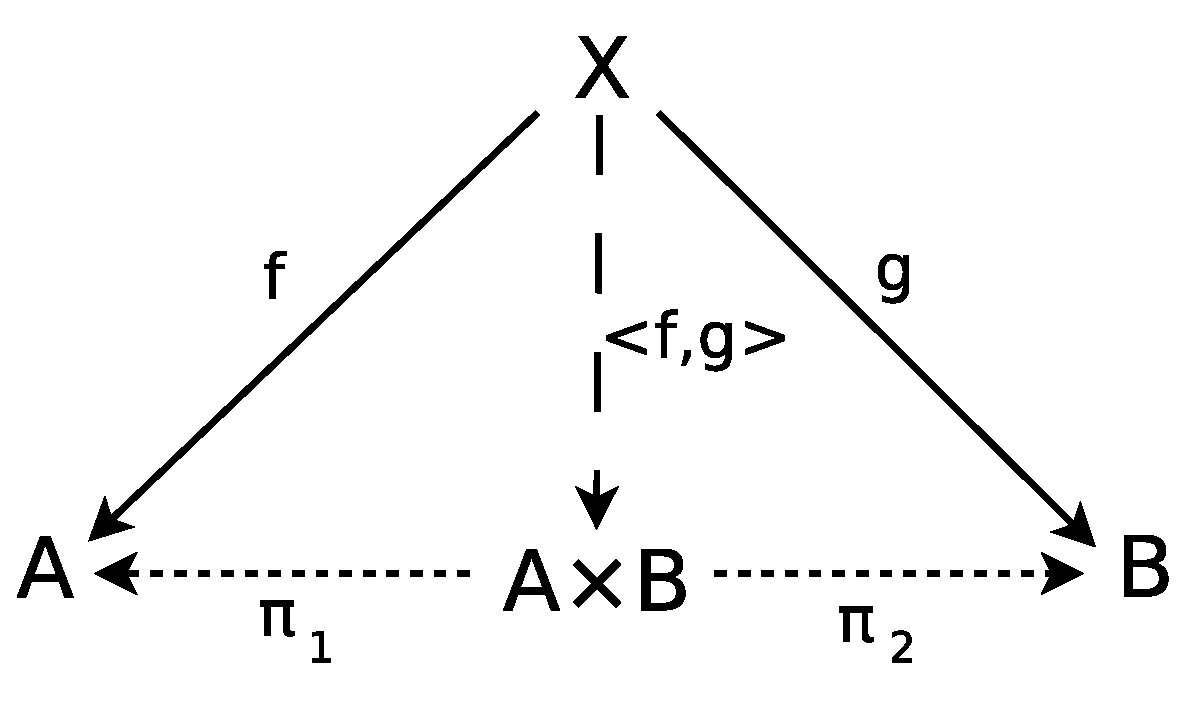
\includegraphics[scale=0.3]{images/cat_product}
    \label{magicl:fig:cat_product}
  }
  \subfloat[Coprodukt]{
    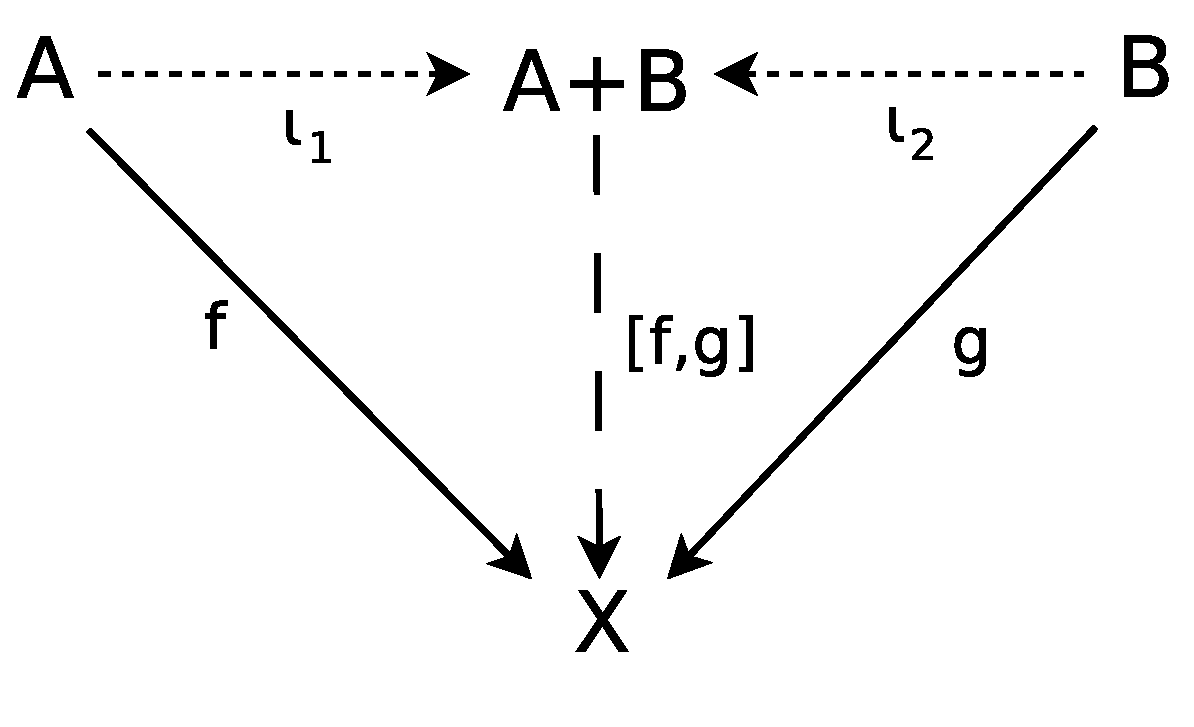
\includegraphics[scale=0.3]{images/cat_coproduct}
    \label{magicl:fig:cat_coproduct}
  }
  \caption{Kommutative Diagramme zur Definition von Produkt und Coprodukt}
\end{figure}

Man kann leicht nachvollziehen, dass das kartesische Produkt genau ein
Produkt für die Kategorie $\mathbf{Set}$ ist. Dreht man im Diagramm alle
Pfeile um, erhält man die Definition für das Coprodukt, ein zum Produkt
dualer\footnote{Die zu einer Kategorie $\mathbf{C}$ duale Kategorie
  $\mathbf{C}^{\mathrm{op}}$ entsteht nämlich durch das Umdrehen von
  Pfeilen.} Operator:

\begin{defi}[Coprodukt]
  Ein Objekt $A + B$ mit zwei Injektionsmorphismen $\iota_1
  \in \mathrm{Mor}_{A,A + B}$ und $\iota_2 \in \mathrm{Mor}_{B,A +
    B}$ ist ein Coprodukt von $A$ und $B$, wenn für jedes $X \in
  \mathrm{Ob}$ und alle $f \in \mathrm{Mor}_{A,X},g \in
  \mathrm{Mor}_{B,X}$ genau ein Morphismus
  $[f,g] \in \mathrm{Mor}_{A + B,X}$ existiert, für den \abb{cat_coproduct} kommutiert, d.h. 
  $[f,g] \circ \iota_1 = f$ und $[f,g] \circ \iota_2 = g$ gelten.
\end{defi}

% \begin{frame}{Kategorien in dieser Arbeit}
%   \begin{itemize}
%   \item Hier immer: Haskell-Datentypen als Objekte
%   \item Arrows variieren:
%     \begin{itemize}
%     \item pure Funktionen (Kategorie $Hask$)
%     \item Funktionen mit Side-Effects
%     \item Bestehende Arrows mit versteckten Ein- und Ausgaben
%     \end{itemize}
%   \end{itemize}
% \end{frame}

% \begin{frame}{Ziel: Eine Parser-Kategorie}
%   \begin{itemize}
%   \item Eigenschaften von Parsern:
%     \begin{itemize}
%     \item Können fehlschlagen und Alternativen ausdrücken
%     \item Besitzen einen Zustand (Position im Eingabestream)
%     \end{itemize}
%   \item Plan: Bestehende Kategorien um Fehlschlagen / Zustände erweitern \\
%   $\Rightarrow$ Funktoren
%   \end{itemize}
% \end{frame}

% \begin{frame}{Der Funktor Fail}
%   \begin{itemize}
%   \item Nun zwei Möglichkeiten für Rückgabe:
%     \begin{itemize}
%     \item Scheitern (Rückgabe einer Fehler-Nachricht)
%     \item Erfolg (normaler Rückgabewert)
%     \end{itemize}
%   \item Verstecken der Veränderung: Neue Kategorie $C_{f}$
%   \item $f_{f} : A \rightarrow B$ wird abgebildet auf
%     $f : A \rightarrow String + B$
%   \item Der Arrow $fail_{f} : String \rightarrow a$ in $C_{f}$ schlägt immer
%     fehl und entspricht $fail : String \rightarrow String + a$ in $C$
%   \item Der Operator $\bigvee : Mor_{A,B} \times Mor_{A,B} \rightarrow
%     Mor_{A,B} $ bietet Alternativen
%   \end{itemize}
% \end{frame}

% \begin{frame}{Der Funktor Fail (2)}
%   \begin{itemize}
%   \item Komposition in $C_{f}$:  $g_{f} \circ f_{f} = ([fail,g] \circ f)_{f}$ 
%   \end{itemize}
%   \begin{figure}
%     \centering
%     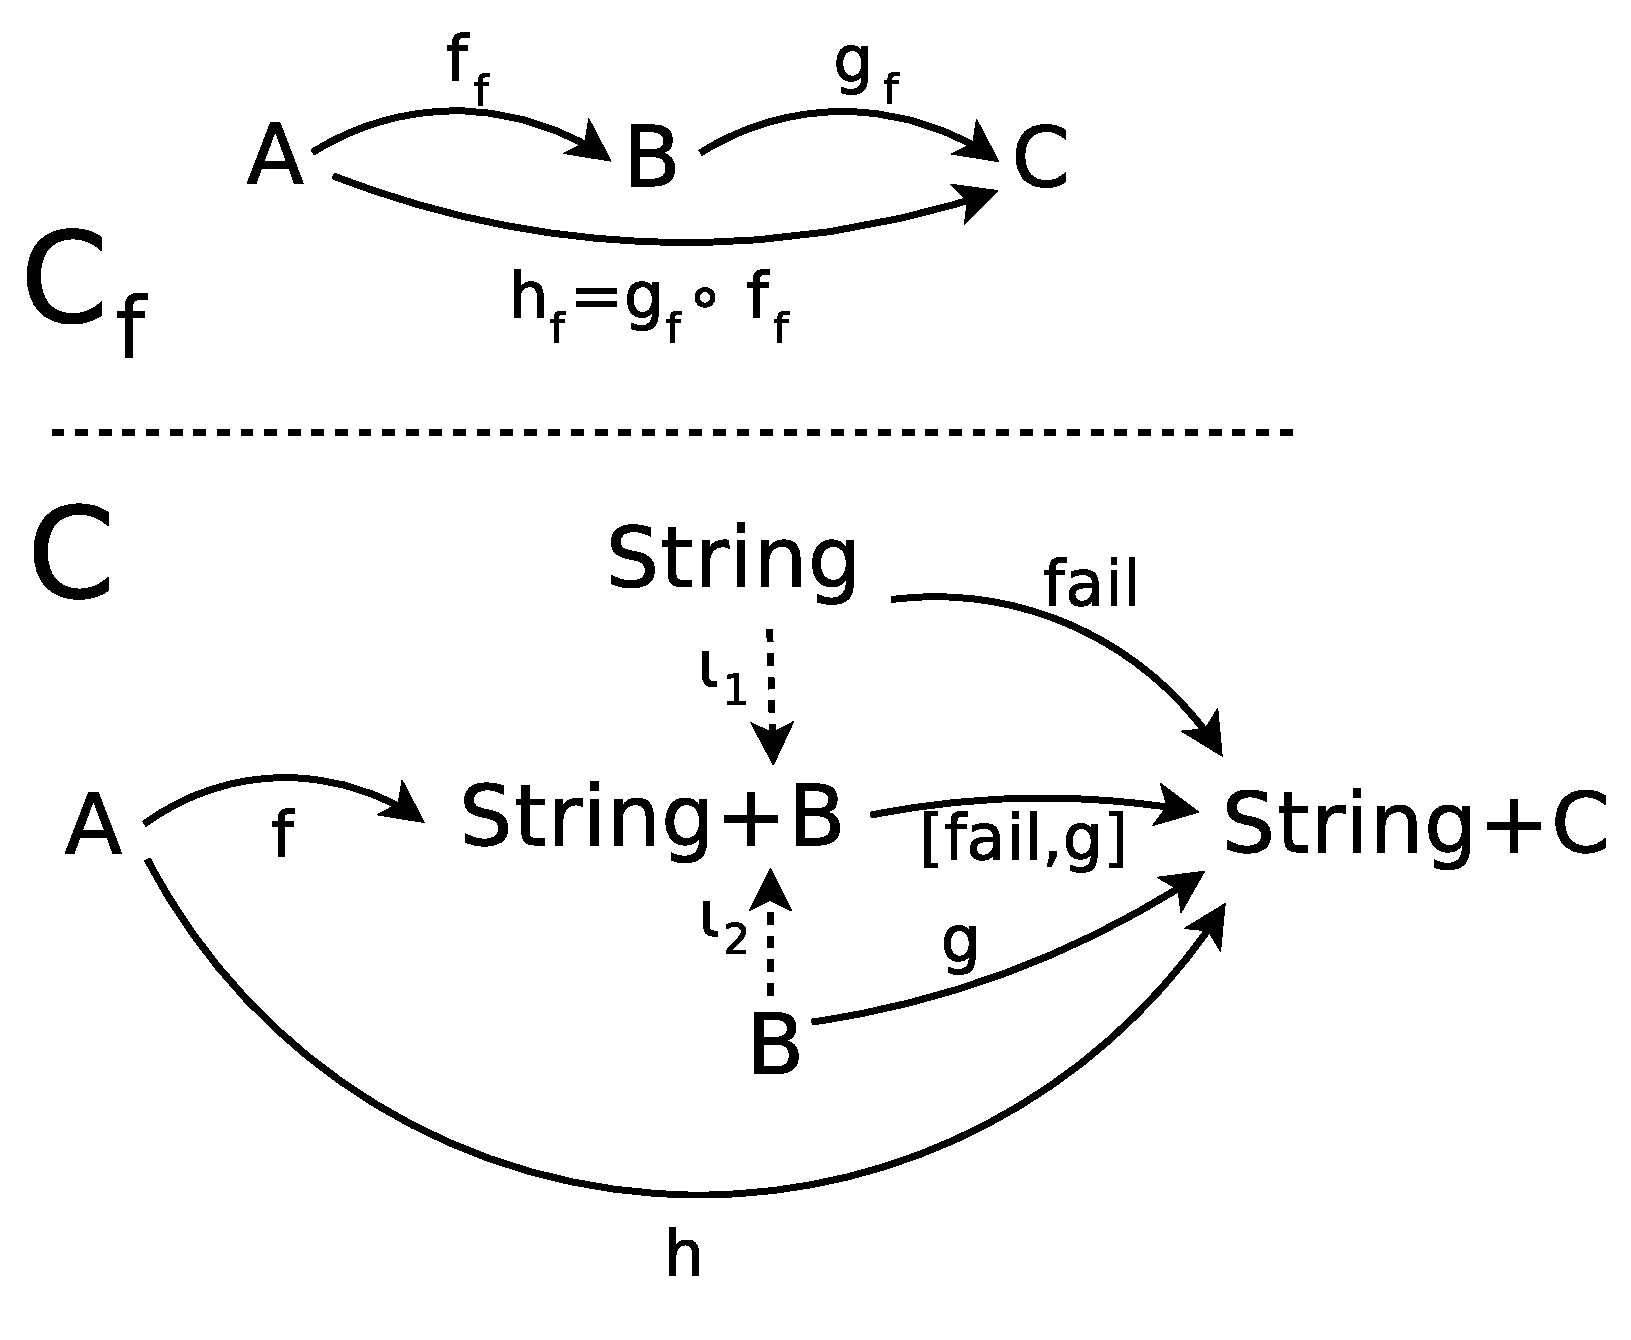
\includegraphics[scale=0.3]{images/cat_fail}
%     \caption{Komposition beim Fail-Funktor}
%   \end{figure}
% \end{frame}

% \begin{frame}{Der Funktor State}
%   \begin{itemize}
%   \item Nun sollen Zustände vom Typ S weitergereicht werden
%   \item Wieder verstecken, neue Kategorie $C_{s}$ mit Funktor
%     $State : C_{s} \rightarrow C$
%   \item $f_{s} : A \rightarrow B$ wird abgebildet auf
%     $f = A \times S \rightarrow B \times S$
%   \item Komposition in $C_{s}$ einfach
%     \begin{figure}
%       \centering
%       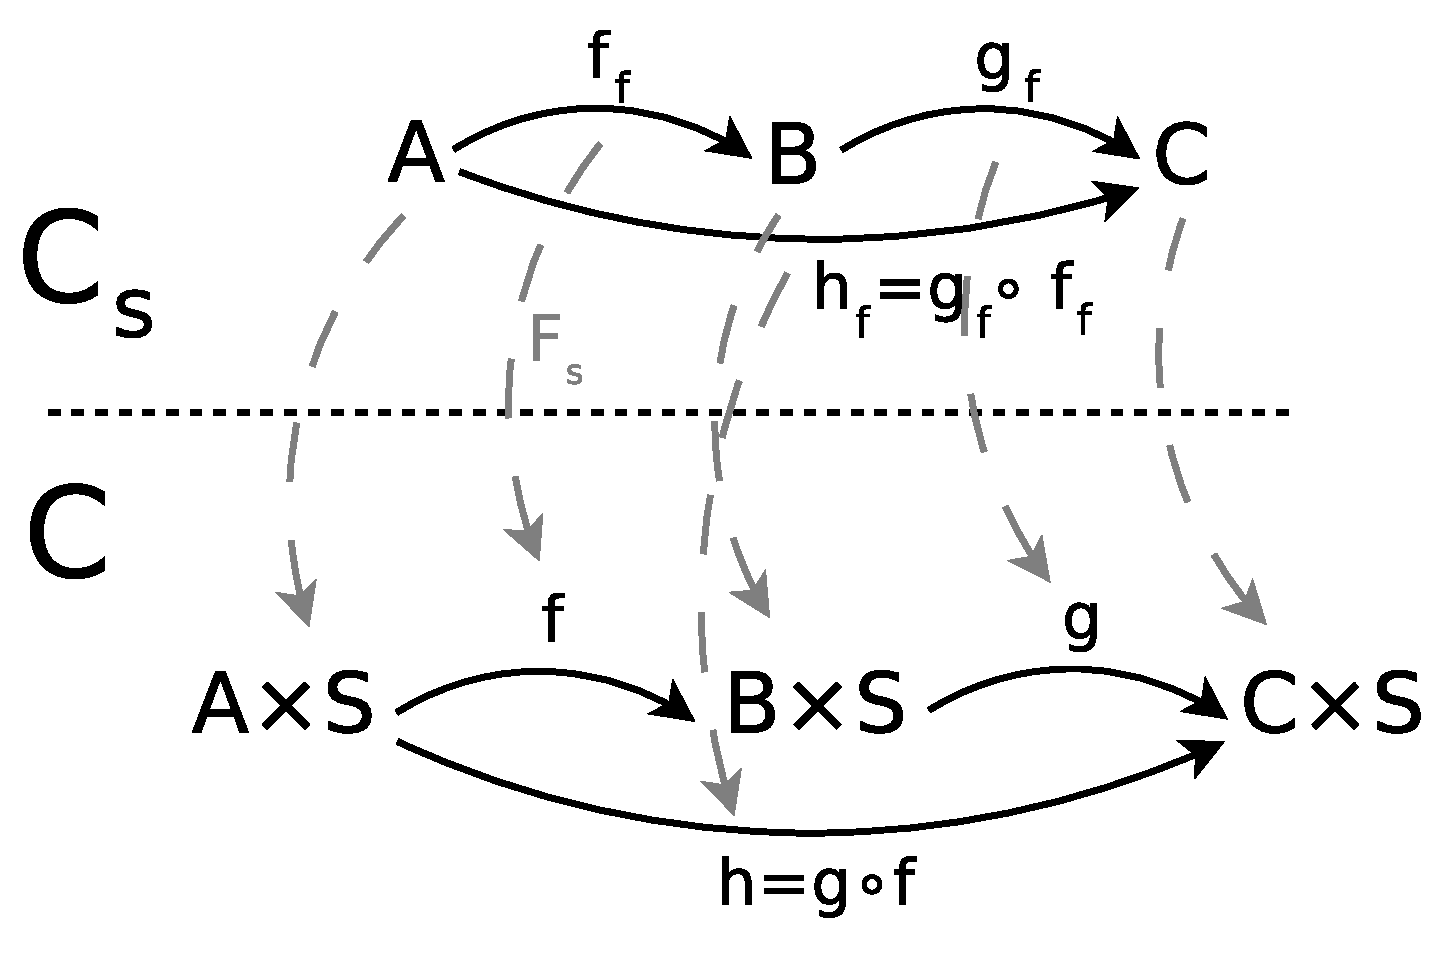
\includegraphics[scale=0.2]{images/cat_state}
%       \caption{Komposition beim State-Funktor}
%     \end{figure}
%   \end{itemize}
% \end{frame}

% \begin{frame}{Der Funktor State (2)}
%   \begin{itemize}
%   \item Etwas Tricky: Produkte in $C_{s}$
%   \item Arbeiten mit Zuständen: Lesen \& Schreiben:
%   \item Lesen: $get_s : \forall a : a \rightarrow S$
%   \item Schreiben: $put_s : S \rightarrow *$
%   \item Zum Parsen: $S = List$ $of$ $T$ mit Token-Typ $T$
%   \end{itemize}
% \end{frame}

% \begin{frame}{Der Parse-Funktor}
%   \begin{itemize}
%   \item Kombination von Fail und State zu einem Funktor Parse
%   \item $C_p = C_{ffs}$
%   \item Zwei Fail-Funktoren für bessere Fehlermeldungen
%   \item Beispiel:
%     \begin{itemize}
%     \item Grammatik: \texttt{\{.*\} $\bigvee$ [.*]}
%     \item Eingabewort: \texttt{\{ABC}
%     \item Schlecht: \texttt{"'Expected [, got \{"'}
%     \item Gut: \texttt{"'Expected \}, got end of stream"'}
%     \item Scheitern nach \texttt{\{} soll Backtracking aushebeln \\
%       $\Rightarrow$ \textit{innerer Fail}
%     \end{itemize}
%   \end{itemize}
% \end{frame}

% \begin{frame}{Der Parse-Funktor (2)}
%   \begin{itemize}
%   \item Flexible Parser-Anwendungen dank Funktor
%     \begin{itemize}
%     \item Funktionale Parser: $Hask_p$
%     \item Parser mit Side-Effects: $IO_p$
%     \item Parser mit anderen Extras: Weitere Funktoren möglich
%     \end{itemize}
%   \item Token-Typ Variabel:
%     \begin{itemize}
%     \item \texttt{Char} für Textdateien
%     \item \texttt{Bool} für Bytestreams
%     \item \texttt{Sexp} für S-Expressions
%     \end{itemize}
%   \item Parser-Bibliothek enthält dazu:
%     \begin{itemize}
%     \item Praktische Funktionen zum Parser-Erzeugen (Blick in \texttt{Parser.hs})
%     \item Möglichkeiten zum Aufruf von inneren Parsern
%     \item Konzepte zum Verschalten von Parsern und Compilern
%     \end{itemize}
%   \end{itemize}
% \end{frame}

% \begin{frame}{Parsen von S-Expressions}
%   \begin{itemize}
%   \item Besonderheit: Token können selbst Listen sein
%   \item Lösung: Als Stream behandeln, \texttt{compNode} wendet Parser
%     auf inneren Stream an
%     \begin{itemize}
%     \item Beispiel: Lesen von \texttt{(hallo welt)}
%     \item \texttt{compNode (symeq "'hallo"' >>> symeq "'welt"') } % <<
%     \end{itemize}
%   \item Makros: \texttt{compNode mit Prüfung des ersten Symbols}
%     \begin{itemize}
%     \item obiges Beispiel: \texttt{macro "'hallo"' (symeq "'welt"')}
%     \item Stimmt das erste Symbol überein, wird das Backtracking aufgehoben
%     \end{itemize}
%   \end{itemize}
% \end{frame}

\end{document}
